\documentclass[a4paper,11pt]{article}
\usepackage[T1]{fontenc}
\usepackage[utf8]{inputenc}
\usepackage{lmodern}
\usepackage{graphicx}
\usepackage{subcaption}
\usepackage{float}
%\usepackage[showframe]{geometry}
\usepackage{layout}

\setlength{\voffset}{-0.75in}
\setlength{\parindent}{0mm}

\title{Hovering@Home Project Description}
\author{Vikas Agrawal}

\begin{document}%\layout

\maketitle
\tableofcontents

\pagebreak

\section{Overview}

The project is divided into 4 teams:
\begin{enumerate}
    \item Control Application Team
    \item Embedded Software Team
    \item Virtual Reality Team
    \item Android Team
    \item Interface Android + Embedded
    \item Interface Embedded + Control
    \item Interface Control + Virtual Reality

\end{enumerate}

\pagebreak

\section{Control Application Team}

The job of the control application team is to make a model through which the HElikopter can
hover. Therefore the team should make a Hovering@Home Model in Matlab.

The Core Quadrocopter Model has the information about the weight, length of the arms and the number of rotors and hence can emulate the Quadrocopter dynamics.
The inputs to the main Quadrocopter model are the initial values of angles, acceleration and the rotor speed.
Through these initial values, the Core Quadrocopter model, calculates the \textbf{subsequent} raw, pitch and yaw angles and also the linear acceleration in all the vectors.

The angles and accelerations are then fed to the Hovering model. The job of this models is to maintain the final set point of all angles ( raw, pitch and yaw = 0 i.e hover ), and thereby calculate the rotor angular speed to be fedback to the Quadrocopter model again. 

This process is done iteratively for the entire time the simulation is running.

Additionally, the control team should generate the Hovering Model using the Real time code generator and verify the  software by means of Software in Loop Tests.


\begin{figure}[ht]
\begin{subfigure}{0.5\textwidth}
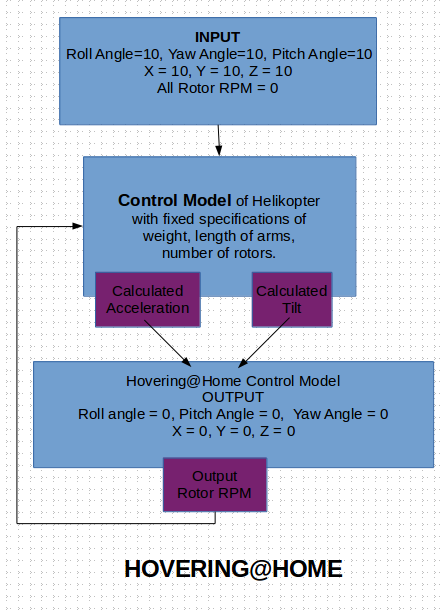
\includegraphics[scale=0.5]{pics/Control1.png}
\end{subfigure}
\begin{subfigure}{1\textwidth}
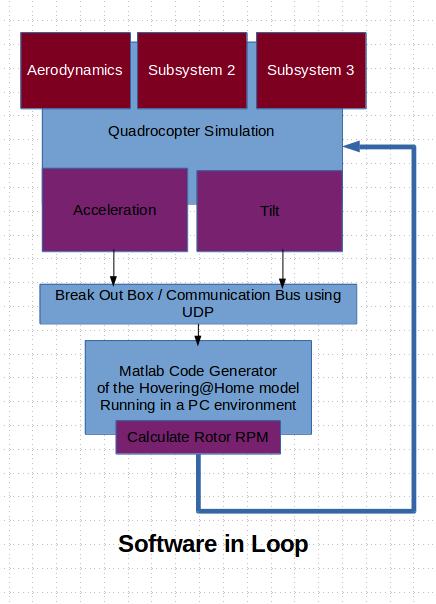
\includegraphics[scale=0.5]{pics/Control2.png}
\end{subfigure}
\end{figure}
 
\pagebreak

\section{Embedded Software Team}

The goal is to build a raspberry image from scratch.
The main goal of this team is to make a stable Real time kernel. Hence a real time linux image needs to be ported to the raspberry hardware. Before the linux image ( kernel.img ) is ported, it is required to also install a bootloader that will boot the kernel.img during the start up process. 

Once the kernel is running, the embedded software team should be able to debug the kernel through GDB. That means the kernel should be compiled with the -ggdb3 ( debug option switched on ).

To be able procure acceleration, magenetic and gyroscope values on the raspberry hardware, IMU, Gyroscope and Magnetic sensor are embedded onto the main raspberry motherboard. The communication between the main raspberry motherboard and the additional board ( consisting of the sensors ) happens over the I2C bus. 

The team should be able to hence build a kernel called HochschuleEsslingenRaspbian.img that already has all the inbuilt packets including the I2C packages.

The application software HElikopter.bin is already provided to you. This application software is already provided to you. The application software can already read the acceleration, magnetic and Gyroscope values. The team should be able to set a breakpoint anytime in the software during the execution of the application software on the hardware to read the internal variables.

\begin{figure}[ht]
\centering
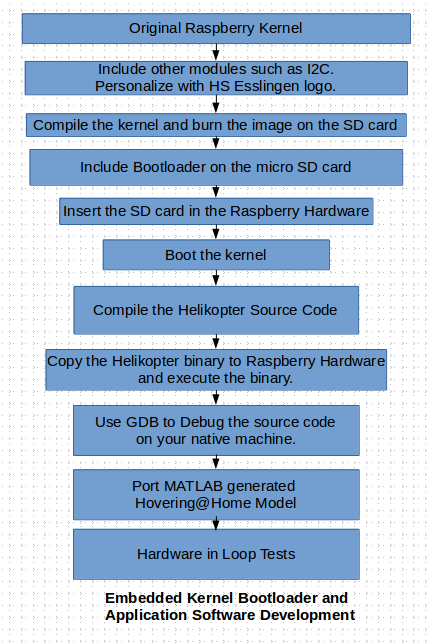
\includegraphics[scale=0.4]{pics/Embedded.png}
\end{figure}

\pagebreak
\section{Virtual Reality Team}


A native software similiar to the Matlab needs to be built in VREP. Here, the specifications are the same as for the Matlab Team. The only difference is that in VREP, the Quadrocopter Dynamics Model is readily available ( drag and drop ), whereas in MATLAB, a Quadrocopter Dynamics Model had to be built from scratch. Also, in V-REP one can attach the sensors ( drag and drop ) on the Virtual Quadrocopter and simply start acquiring the values, once the system is run.

\begin{figure}[ht]
\centering
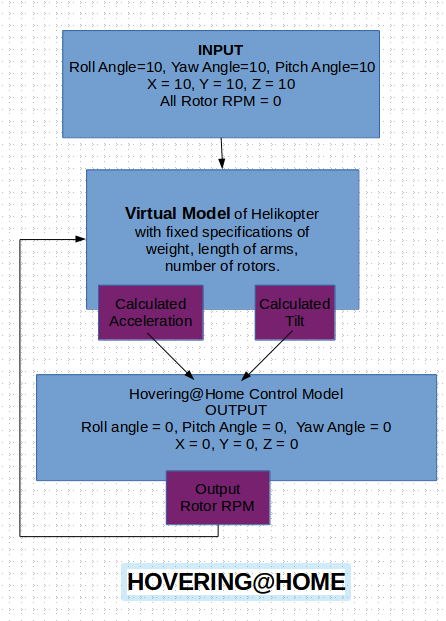
\includegraphics[scale=0.5]{pics/VirtualReality.png}
\end{figure}

\pagebreak
\section{Android Team}

TODO

\pagebreak
\section{Interface between Android and Embedded Software }

TODO


\pagebreak
\section{Interface between Embedded Software and Control Application }

Ofcourse, even if raspberry and the control simulations are available, the quadrocopter body ( or basically the whole car ) is not available for tests. In our case, yes, but if you would have been a Tier II supplier, it would not have been available immediately to you. So, lets assume that we do not have any Quadrocopter body as of now.

The following method to test the embedded software even if the real car is not available is called Hardware in the Loop Tests. We need a hardware in the Loop simulation which is everything from the Control Team except the Hovering Model. This is self explanatory, because the developed Hovering Model under MATLAB is already ported to the Embedded hardware.

\begin{figure}[ht]
\centering
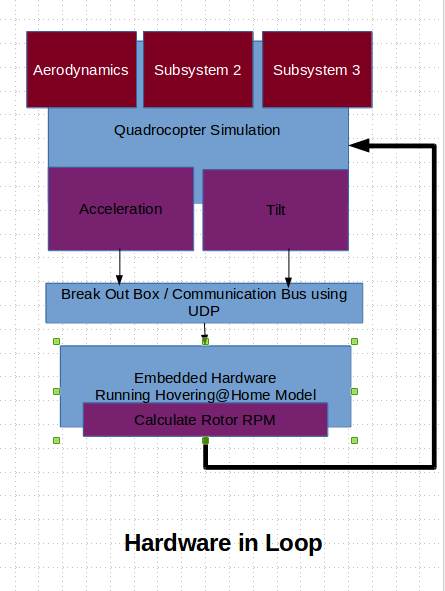
\includegraphics[scale=0.5]{pics/Interface-Control-Embedded.png}
\end{figure}

\pagebreak

\section{Interface between Control Application and Virtual Reality}

The MATLAB software already runs the Hovering@Home model. In this model, the quadrocopter always has to return at 0,0,0 and hover at an altitude of 1 m. Any kind of disturbances for example pushing the quadrocopter with the hand or due to wind, must bring the Quadrocopter back to 0,0,0.

The VR team should prepare a validation software. One of the use cases in the validation software is for example, to change the (x,y,z) position of the quadrocopter and see if the quadrocopter returns to its original position 0,0,0.
The changes should be ofcourse visible graphically in a 3D environment.

\begin{figure}[ht]
\centering
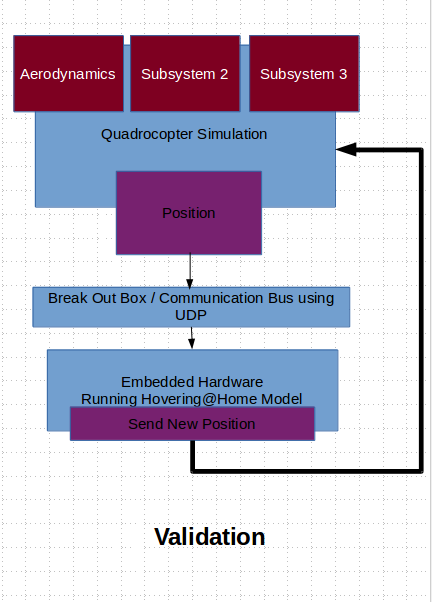
\includegraphics[scale=0.5]{pics/Interface-Control-VR.png}
\end{figure}


\end{document}
